\documentclass[12pt,oneside]{article}
\usepackage[margin=1in]{geometry}
\usepackage{minted}
\pagenumbering{gobble}
\usepackage{amssymb,amsmath,amsthm}
\renewcommand{\baselinestretch}{1.1}
\renewcommand{\arraystretch}{.91}
\usepackage{graphicx}
\usepackage{pdfpages}

% Define an environment for exercises.
\newenvironment{exercise}[1]{\vspace{.5cm}\noindent\textbf{#1 \hspace{.05em}}}{}

% Allow for underlining.
\usepackage[normalem]{ulem}

% define shortcut commands for commonly used symbols
\newcommand{\R}{\mathbb{R}}
\newcommand{\C}{\mathbb{C}}
\newcommand{\Z}{\mathbb{Z}}
\newcommand{\Q}{\mathbb{Q}}
\newcommand{\N}{\mathbb{N}}
\newcommand{\lr}[1]{\left( #1 \right)}
\newcommand{\lrb}[1]{\left[ #1 \right]}
\newcommand{\lrc}[1]{\left{ #1 \right}}
\newcommand{\eq}[1]{\begin{align*}#1\end{align*}}
\newcommand{\degs}{\ensuremath{^\circ}}
\newcommand{\abs}[1]{\lvert#1\rvert}
\newcommand{\ohm}{\ensuremath{\Omega}}
\newcommand{\sci}{\times 10^}
\newcommand{\calP}{\mathcal{P}}

\DeclareMathOperator{\vsspan}{span}

%%%%%%%%%%%%%%%%%%%%%%%%%%%%%%%%%%%%%%%%%%

\begin{document}

\setlength{\belowdisplayskip}{5pt} \setlength{\belowdisplayshortskip}{0pt}
\setlength{\abovedisplayskip}{-10pt} \setlength{\abovedisplayshortskip}{0pt}

\begin{flushright}
Matthew Burns \\
William Fedus \\
Bobak Hashemi \\
April 17, 2015 \\
\end{flushright}


% --------------------------------- Title Header
\begin{center}
CSE 291 Project 1\\
\emph{An application of linear regression to predict housing prices}
\end{center}
% --------------------------------- End Title

\begin{flushleft}
% --------------------------------- Begin MinFunc Implementation
\subsection*{Problem Definition}
We are given a list of $m$ ``features" and the sale price for $N$ homes. The features are decimal numbers which characterize physical information about the property. We assume that the features have been picked carefully enough that they contain the necessary information to estimate the value of each home. Under this model, the sale price of the home is 

\begin{equation}
s = h(\vec{x}) + \epsilon
\end{equation} \newline

where $h(\vec{x})$ is the intrinsic value of the property, a function of the chosen features. $\epsilon$ is the perturbation to the intrinsic value, which is a function of a broad number of additional variables that are random in nature and can be modeled as Gaussian noise with $\sigma << \abs{h}$.  

The simplest approximation to $h(\vec{x})$ is a linear function of the form 

\begin{equation}
h(\vec{x}) \approx \omega_0 + \omega_1 x_1 + ... + \omega_n x_n
\end{equation}\newline

In the following sections we will document a set of implemented scripts which find the ``best" approximation to $h(\vec{x})$, in Matlab, given that we restrict ourselves to a linear function of the features. 
% --------------------------------- End Problem Definition
% --------------------------------- Begin Preprocessing

\subsection*{Preprocessing}
We shall denote the vector of the weights $\omega_i$ as $\vec{\theta}$, and the vector of features for the $i$th property as $\vec{x}_i$. We construct the $N\times(m+1)$ dimensional matrix, $X$, using the definition

\begin{equation}
X = \begin{bmatrix}
1 & \vec{x}_1 \\
... \\
1 & \vec{x}_N
\end{bmatrix},
\end{equation}\newline
so that $h(\vec{x}_i)$ is the $i$th row of $X\vec{\theta}$. Finally, the sale prices for the $i$th house $y_i$ are combined in the $N$ dimensional vector $\vec{y}$.


% --------------------------------- End Preprocessing
% --------------------------------- Begin MinFunc Implementation
\subsection*{MinFunc Implementation}
Minfunc is a Matlab package for optimizing real valued multi-variate functions. The minfunc function call takes in $\vec{\theta}$, $\vec{y}$, $X$, and a custom function that returns a tuple $[f,g]$, where $f$ is the objective function and $g$ is the gradient of $f$ with respect to $\vec{\theta}$. minfunc returns an optimized $\vec{\theta}$, in ex1a\_linreg.m:

\begin{minted}{matlab}
[alltheta{1}] = minFunc(@linear_regression, theta, options, train.X, train.y);
\end{minted}

We have named our custom function linear\_regression.m in this example.

The next step is to define a simple objective function, one choice is the squared 2-norm: 

\begin{equation}
f = \left \| X\vec{\theta} - \vec{y} \right \|_{2}^2
\end{equation}

\begin{equation}
g = \nabla_{\vec{\theta}} f =  2\vec{\theta}^T X^T X - 2\vec{y}^T X
\end{equation}\newline 

These definitions are implemented in linear\_regression.m:

\begin{minted}{matlab}
  e=y'-X'*theta;
  f=e'*e; % Euclidean norm squared between targets and guess
  g=2*(X*X')*theta-2*(y*X')'; % Gradient of the objective 
\end{minted}

% --------------------------------- End MinFunc Implementation    
% --------------------------------- Begin Gradient Descent
\subsection*{Gradient Descent}
Gradient descent is a first order linear optimization algorithm which finds a local minima in a function $f$ by stepping in the direction of the negative gradient of the function.  In particular, the update rule is given by Equation \ref{eqn: grad_desc},

\begin{equation}\label{eqn: grad_desc}
\vec{\theta_{t+1}} = \vec{\theta_t} - \eta(t) \nabla f
\end{equation}\newline

\noindent where $\vec{\theta}$ is the parameter vector we seek which is a local minima of $f$ and $\eta(t)$ is the step size at iteration $t$.  In a simplest format, $\eta_t$ may be chosen to be a constant value, that is, the algorithm will take a constant step size at each iteration.  However, for step sizes too small, convergence may be excessively slow and for step sizes too large, convergence may be an issue since the algorithm may overstep the equilibrium.  In order to solve this issue, we use the backtracking algorithm to reduce $\eta_t$ as we perform gradient descent.  


% --------------------------------- End Gradient Descent
% --------------------------------- Begin Closed Form Solution
\subsection*{Closed Form Solution}

$f$ is quadratic function of the parameters $\omega$ that is always greater than $0$. These two facts guarantee the existence of a unique minimum for $E$ with respect to $\vec{\theta}$. We define the optimal $\vec{\theta}'$ as the one which minimizes the expression

We know this objective function f is convex because it is a norm, so any stationary point is guaranteed to be a local minimum. Setting $g=0$ in (5) and solving for $\vec{\theta}$: 

\begin{equation}
\hat{\vec{\theta}}=(X^T X)^{-1}X^T\vec{y}
\end{equation}

\begin{minted}{matlab}
function [theta, f, g, exitflag ] = closed_form( X, y )
theta=X*X'\X*y';
end
\end{minted}

\subsection*{Results}
All three methods converged, with the gradient descent taking the most iterations (10,000). We compare the performance of the three methods via Root Mean Squared Error over the partitioned test set.  We display the results of the three methodologies in Table \ref{tab:performance}.

\begin{table}[h!]
\centering
 \begin{tabular}{| c | c|} 
 \hline
   Measure & RMSE\\ [0.7ex] 
 \hline\hline
  MinFunc & 5.03  \\ 
  \hline
  Gradient Descent & 5.81  \\  [1ex] 
 \hline
  Closed Form Solution & 5.03  \\  [1ex] 
 \hline
 \end{tabular}
 \caption{Performance of our three approaches as measured by RMSE on the partitioned test set.}
\label{tab:performance}
\end{table}

\pagebreak 
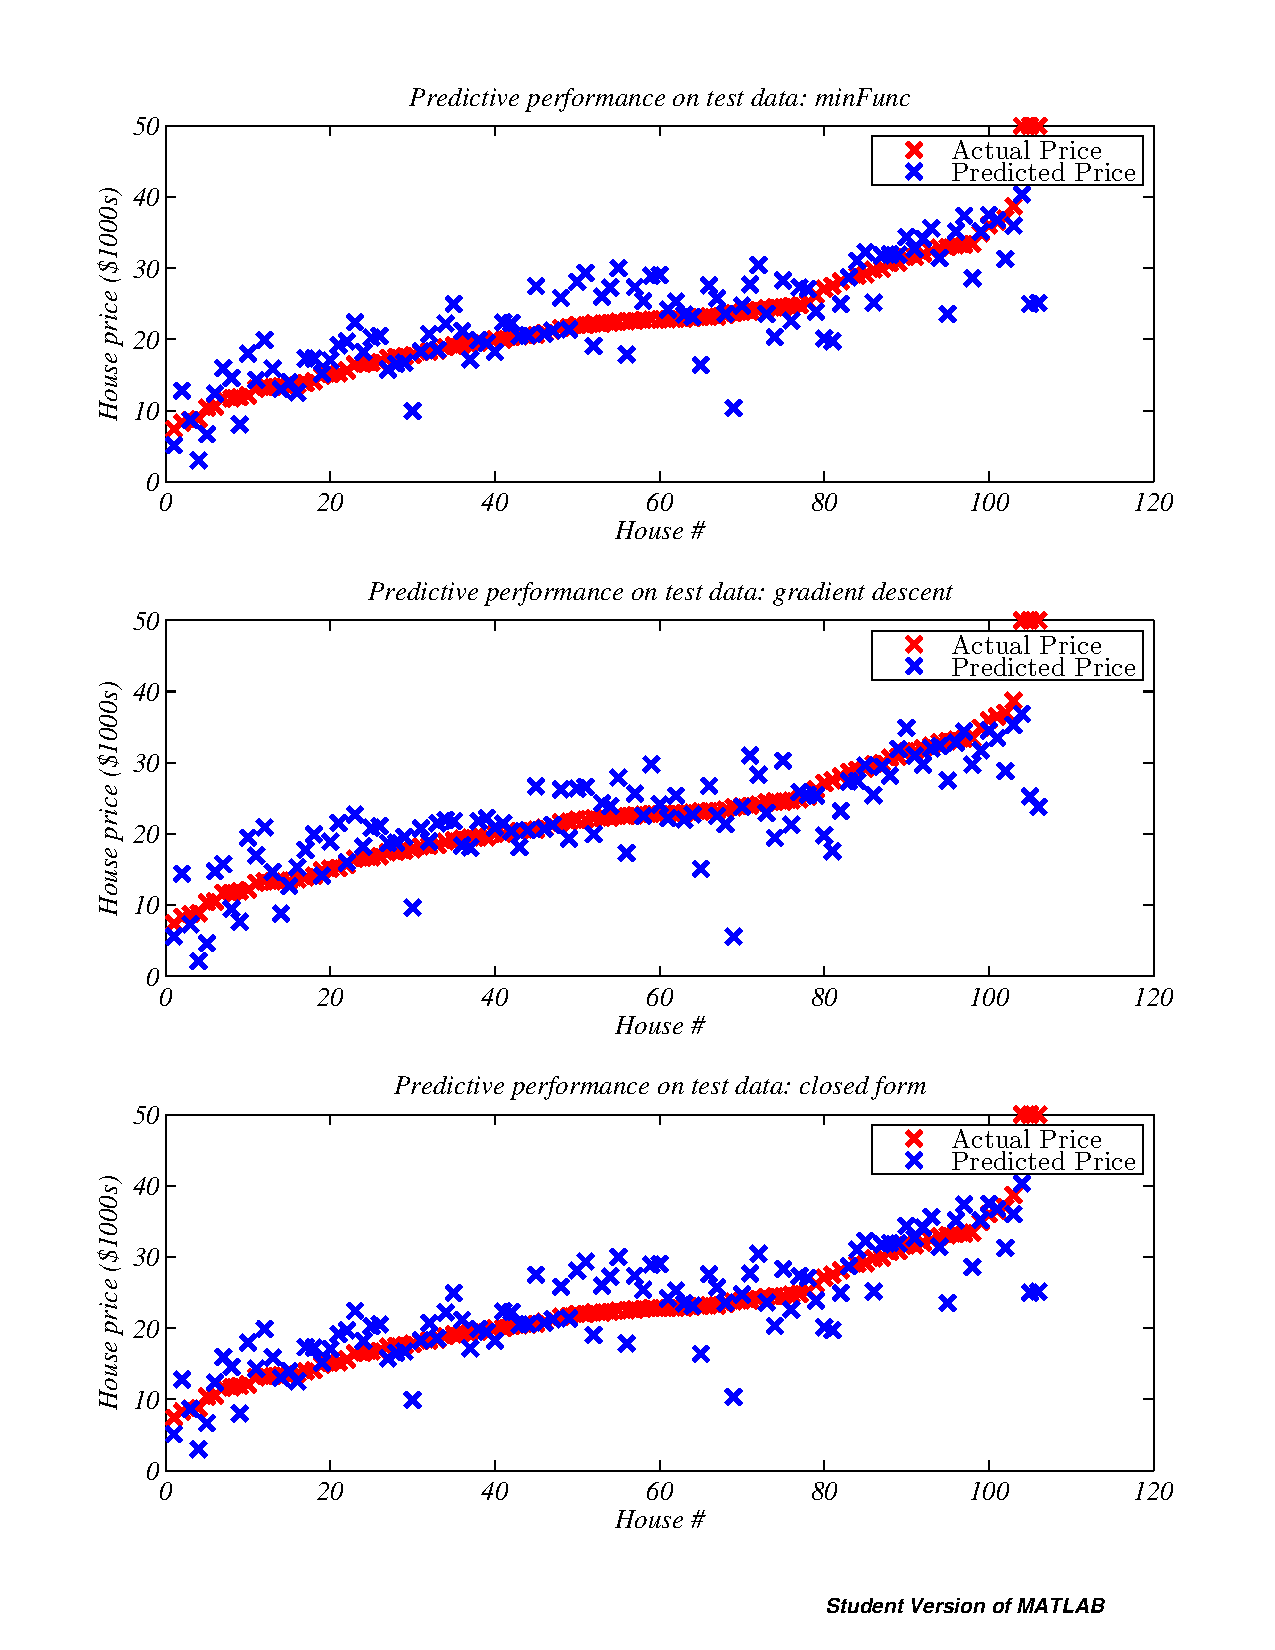
\includepdf[pages={1}]{Predictive_Performance.pdf}

\subsection*{Who did what?}
\textbf{Matt}: Closed form solution, solution and code\\
\textbf{William}: Gradient descent, solution and code\\
\textbf{Bobak}: Code manager, LaTeX, theoretical development\\


% --------------------------------- End Closed Form Solution


\begin{thebibliography}{9}

\bibitem{Linreg}
  Matthew Burns, Bobak Hashemi, William Fedus, Computer Code, extending the original work of Bache, K. \& Lichman, M. (2013). UCI Machine Learning Repository. URL: \emph{https://github.com/bth5032/CreamCastle\_CSE291/tree/master/project\%201}

\bibitem{minfunc}
Schmidt, M. (2005). MinFunc. Retrieved April 14, 2015, from http://www.cs.ubc.ca/~schmidtm/Software/minFunc.html
\end{thebibliography}


\end{flushleft} 
\end{document}